\documentclass[tikz,border=2pt]{standalone}
\usepackage{amsmath,amssymb}
\usepackage{tikz}
\usetikzlibrary{arrows.meta}

\begin{document}
% A subspace U is invariant under A when A maps U into itself: the x1-axis is invariant under
% A = [[2,1],[0,3]] (an eigen-line), the x2-axis is not.
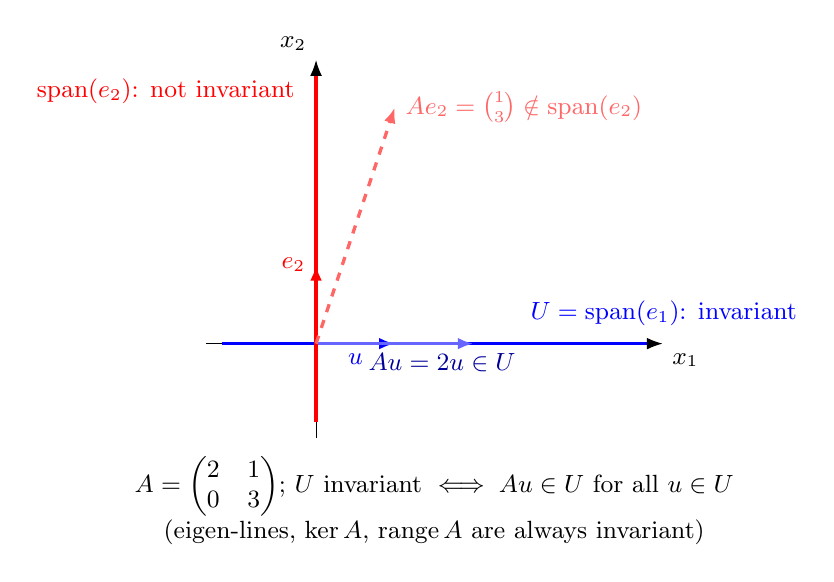
\begin{tikzpicture}[every node/.style={font=\small}, >={Latex[length=2mm]}]
	\draw[->] (-1.4,0) -- (4.4,0) node[below right] {$x_1$};
	\draw[->] (0,-1.2) -- (0,3.6) node[above left] {$x_2$};
	\draw[blue, very thick] (-1.2,0) -- (4.2,0);
	\node[blue, anchor=south west] at (2.6,0.1) {$U=\operatorname{span}(e_1)$: invariant};
	\draw[->, blue, very thick] (0,0) -- (1,0);
	\node[blue, below, font=\small] at (0.5,0) {$u$};
	\draw[->, blue!60, very thick] (0,0) -- (2,0);
	\node[blue!60!black, below, font=\small] at (1.6,0) {$Au=2u\in U$};
	\draw[red, very thick] (0,-1.0) -- (0,3.4);
	\node[red, anchor=east] at (-0.15,3.2) {$\operatorname{span}(e_2)$: not invariant};
	\draw[->, red, very thick] (0,0) -- (0,1) node[left, font=\small] {$e_2$};
	\draw[->, red!60, very thick, dashed] (0,0) -- (1,3) node[right, font=\small] {$Ae_2=\binom13\notin\operatorname{span}(e_2)$};
	\node[anchor=north, align=center] at (1.5,-1.3) {$A=\begin{pmatrix}2&1\\0&3\end{pmatrix}$; $U$ invariant $\iff Au\in U$ for all $u\in U$\\ (eigen-lines, $\ker A$, $\operatorname{range}A$ are always invariant)};
\end{tikzpicture}
\end{document}
